\chapter{ចរន្តអគ្គិសនី រេស៊ីស្ទង់ និងកម្លាំងអគ្គិសនីចលករ}
\begin{center}
	{\Large \kml\color{magenta}មេរៀនសង្ខេប}
\end{center}
\section{អានុភាព និងថាមពល}
\begin{enumerate}[k,2]
	\item អានុភាពអគ្គិសនី $P_{e}=VI$
	\item ថាមពលអគ្គិសនី $W_{e}=P_{e}t=VIt$
\end{enumerate}
\section{អង្គធាតុចម្លង់អូម}
\begin{enumerate}[k]
	\item តង់ស្យុងរវាងគោលអង្គធាតុចម្លងអូម $V=RI$
	\item អានុភាពអគ្គិសនីអង្គធាតុចម្លងអូម $P_{e}=VI=RI^{2}$
	\item ថាមពលអគ្គិសនីអង្គធាតុចម្លងអូម $W_{e}=P_{e}t=VIt=RI^{2}t$
	\item ទិន្នផលអង្គធាតុចម្លងៈ អង្គធាតុចម្លងផ្តល់ទិន្នផល $100\%$
\end{enumerate}
\begin{figure}[H]
	\centering
	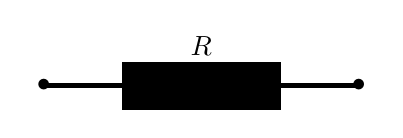
\begin{tikzpicture}
		\draw[line width = 2pt] (0,0) -- (1,0);
		\filldraw (1,-.3) rectangle (3,.3);
		\draw[line width = 2pt] (3,0) -- (4,0);
		\node at (2,.5) {$R$};
		\node at (0,0) {$\bullet$};
		\node at (4,0) {$\bullet$};
	\end{tikzpicture}
	\caption{\DS រេស៊ីស្ទង់ ឬអង្គធាតុចម្លងអូម}
\end{figure}
\section{គ្រឿងទទួលគំរូ(ម៉ូទ័រ និងផើងវិភាគ):} លក្ខខណ្ឌដើម្បីឲ្យគ្រឿងទទួល ដំណើរការៈ $V>E'$
\begin{enumerate}[k]
	\item តង់ស្យុងរវាងគោលគ្រឿងទទួលគំរូៈ $V=E'+Ir'$
	\item អានុភាពអគ្គិសនីគ្រឿងទទួលគំរូៈ $P_{e}=P_{U}+P_{J}=E'I+r'I^{2}$
	\item ទិន្នផលគ្រឿងទទួលគំរូៈ $R_{d}=\frac{W_{U}}{W_{e}}=\frac{P_{U}}{P_{e}}=\frac{E'}{V}$
\end{enumerate}
\begin{figure}[H]
	\begin{subfigure}[t]{0.5\textwidth}
		\centering
		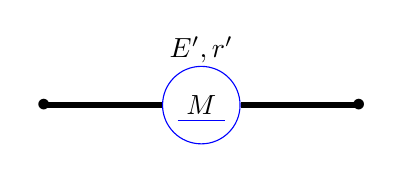
\begin{tikzpicture}
			\draw[line width = 2pt] (0,0) -- (1.5,0);
			\draw[line width = 2pt] (2.5,0) -- (4,0);
			\node at (2,.7) {$E',r'$};
			\node at (2,0) {$M$};
			\node at (0,0) {$\bullet$};
			\node at (4,0) {$\bullet$};
			\draw[blue] (2,0) circle (14pt);
			\draw[blue] (1.7,-.2) -- (2.3,-.2);
		\end{tikzpicture}
		\subcaption{ម៉ូទ័រ}
	\end{subfigure}
	\begin{subfigure}[t]{0.5\textwidth}
		\centering
		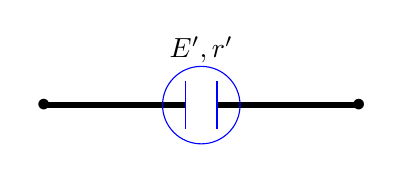
\begin{tikzpicture}
			\draw[line width = 2pt] (0,0) -- (1.8,0);
			\draw[line width = 2pt] (2.2,0) -- (4,0);
			\node at (2,.7) {$E',r'$};
			\node at (0,0) {$\bullet$};
			\node at (4,0) {$\bullet$};
			\draw[blue] (2,0) circle (14pt);
			\draw[blue] (1.8,-.3) -- (1.8,.3);
			\draw[blue] (2.2,-.3) -- (2.2,.3);
		\end{tikzpicture}
		\subcaption{ផើងវិភាគ}
	\end{subfigure}
\end{figure}
\section{ករណីម៉ូទ័រគាំង ឬផើងវិភាគមានបាតុភូតអាណូតរលាយៈ  $V=r'I$}
\section{ជនិតាចរន្តជាប់ៈ(អាគុយ និងថ្មពិល) ភ្លើង $DC$}
\begin{enumerate}[k]
	\item តង់ស្យុងគោលជនិតាចរន្តជាប់ៈ $V=E-Ir$
	\begin{itemize}
		\item បើ $r=0$ នោះ $V=E=$ថេរ ជនិតាជាប្រភពអុីដេអាល់នៃតង់ស្យុង។
		\item បើ $I=0$ នោះ $V=E$ ជាសៀគ្វីចំហរគ្មានចរន្តឆ្លងកាត់។
		\item បើ $V=0$ នោះ $I_{CC}=\frac{E}{r}$(បាតុភូតឆ្លងភ្លើង)
	\end{itemize}
	\item អានភាពអគ្គិសនី នៃជនិតា $P_{g}=P_{e}+P_{J}$
	\begin{flalign*}
		\text{ដែល}\quad: &\quad P_{g}=EI\quad\text{ជាអានុភាពគីមីនៃជនិតាគិតជា $W$}\\
		\quad:&\quad P_{e}=VI\quad\text{ជាអានុភាពអគ្គិសនីបញ្ចេញដោយជនិតាគិតជា $W$} \\
		\quad:&\quad P_{J}=rI^{2}\quad\text{ជាអានុភាពកម្តៅបញ្ចេញដោយជនិតាគិតជា $W$}
	\end{flalign*}
	\item ថាមពលអគ្គិសនី នៃជនិតាៈ $W_{g}=W_{e}+W_{J}$
	\item ទិន្នផលជនិតាចរន្តជាប់ៈ $R_{d}=\frac{W_{e}}{W_{g}}=\frac{P_{e}}{P_{g}}=\frac{V}{E}$
\end{enumerate}
\section{ចំណុះអាគុយ-វដ្តអាគុយៈ}
\begin{enumerate}[k]
	\item អាគុយពេលសាកភ្លើង(បញ្ចូលភ្លើង): $V=E+Ir$
	\item អាគុយពេលប្រើៈ $V=E-Ir$
\end{enumerate}
\section{ចរន្តអគ្គិសនីៈ}
\begin{enumerate}[k]
	\item ចរន្តឆ្លងកាត់ខ្សែចម្លងៈ $I=\frac{q}{t}$
	\item ទំនាក់ទំនង់រវាងចរន្ត និងល្បឿនអេឡិចត្រុងៈ $I=nAve$
\end{enumerate}
\begin{flalign*}
	\text{ដែល}\quad: &\quad n=\frac{V}{N}\quad\text{ជាចំនួនអេឡិចត្រុងក្នុងមួយខ្នាតមាឌ $m^{-3}$}\\
	\quad:&\quad N\quad\text{ជាចំនួនអេឡិចត្រុងសរុបឆ្លងកាត់ផ្ទៃ $A$} \\
	\quad:&\quad V=AL\quad\text{ជាមាឌខ្សែ $m^{3}$}\\
	\quad:&\quad v\quad\text{ជាល្បឿនអេឡិចត្រុង $m/s$}
\end{flalign*}
\begin{center}
	{\Large \kml\color{magenta} ចប់ដោយសង្ខេប!!!}
\end{center}
\newpage
\section{សំណួរ និងលំហាត់អនុវត្ត}
\begin{enumerate}
	\item ខ្សែចម្លងមួយមានប្រវែង $\ell=100m$ មុខកាត់ $A=250mm^{2}$ មានរេស៊ីស្ទីវីតេ $\rho=2.5\times10^{-8}\Omega m$។ \\គណនារេស៊ីស្តង់នៃខ្សែចម្លង។
	\item គណនាប្រវែងខ្សែចម្លងមួយដែលមានរេស៊ីស្តង់ $R=2\Omega$ មានមុចកាត់ $0.1cm^{2}$ និងមានរេស៊ីស្ទីវីតេ \\$\rho=2.5\times10^{-8}\Omega m$។
	\item ខ្សែចម្លងមួយមានអង្កត់ផ្ចិត $d=1mm$ មានប្រវែង $\ell=314m$ ហើយមានរេស៊ីស្ទីវីតេ $\rho=1.6\times10^{-8}\Omega m$។\\ គណនារេស៊ីស្តង់នៃខ្សែចម្លងនេះ។
	\item ប៊ូបីនមួយមានអង្កត៊ផ្ចិត $D=5cm$ រុំនឹងខ្សែចម្លងមួយដែលមានអង្កត៊ផ្ចិត $d=0.8mm$ មានរេស៊ីស្ទីវីតេ \\$\rho=1.6\times10^{-8}\Omega m$ និងមានចំនួនស្ពៀ $1000$ ស្ពៀ។ គណនារេស៊ីស្តង់នៃប៊ូបីន។
	\item គេធ្វើឲ្យចរន្តអគ្គិសនី $I=2A$ ឆ្លងកាត់មុខកាត់នៃខ្សែចម្លងមួយក្នុងរយៈពេល $t=30s$។
	\begin{enumerate}
		\item គណនាបរិមាណបន្ទុកអគ្គិសនីដែលឆ្លងកាត់ខ្សែចម្លង។
		\item គណនាចំនួនអេឡិចត្រុងដែលឆ្លងកាត់ខ្សែចម្លង បើ $\abs{-e}=1.6\times10^{-19}C$
	\end{enumerate}
	\item គណនាល្បឿនអេឡិចត្រុងរត់ក្នុងខ្សែទង់ដែង ដែលមានមុខកាត់ $2mm^{2}$ ឆ្លងកាត់ដោយចរន្ត $2A$។ គេឲ្យម៉ាសម៉ូលនៃខ្សែទង់ដែង $63.5g/mol$ ម៉ាសមាឌទង់ដែង $\rho=8.9\times10^{3}kg/m^{3}$ និងចំនួនអាវ៉ូកាដ្រូ $N_{A}=6.02\times10^{23}$ បើអាតូមនីមួយៗមានអេឡិចត្រុងស៊េរីចំនួនមួយ។
	\item ម៉ូទ័រអគ្គិសនីមួយមានកម្លាំងច្រាសអគ្គិសនីចលករ $E'=24V$ និងរេស៊ីស្តង់ $r'=2\Omega$ ប្រើក្រោមតង់ស្យុង $V=48V$។ គណនាអានុភាពមេកានិចបញ្ចេញដោយម៉ូទ័រ។
	\item គេភ្ជាប់ប៉ូលទាំងពីរនៃជនិតាមួយដែលមានកម្លាំងអគ្គិសនីចលករ $E=12V$ និងមានរេស៊ីស្តង់ក្នុង $r=1\Omega$ ទៅឲ្យម៉ូទ័រអគ្គិសនីមួយដែលមានកម្លាំងច្រាសអគ្គិសនីចលករ $E'=3V$ និងរេស៊ីស្តង់។
	\begin{enumerate}
		\item គណនាអាំងតង់ស៊ីតេចរន្តដែលឆ្លងកាត់សៀគ្វី។
		\item គណនាតង់ស្យុងនៃជនិតា។
	\end{enumerate}
	\item តង់ស្យុងរវាងប៉ូលទាំងពីរនៃជនិតាមួយមានតម្លៃ $V_{1}=10V$ កាលណាវាបញ្ចេញចរន្ត $I_{1}=3A$ ហើយវាមានតង់ស្យុង $V_{2}=8.8V$ កាលណាវាបញ្ចេញចរន្ត $I_{2}=5A$។ គណនាកម្លាំងអគ្គិសនីចលករ $E$ និងរេស៊ីស្តង់ $r$ របស់ជនិតា។
	\item គេភ្ជាប់ប៉ូលទាំងពីរនៃជនិតាមួយដែលមានកម្លាំងអគ្គិសនីចលករ $E=12V$ និងរេស៊ីស្តង់ $r=1\Omega$ ទៅសៀគ្វីក្រៅដែលមានកំសៀវអគ្គិសនីមួយមានរេស៊ីស្តង់ $R=200\Omega$។
	\begin{enumerate}
		\item គណនាអាំងតង់សុីតេចរន្តឆ្លងកាត់សៀគ្វី និងតង់ស្យុងរវាងប៉ូលនៃជនិតា។
		\item គណនាថាមពលអគ្គិសនីស៊ីដោយកំសៀវក្នុងរយៈពេល $30mn$។
	\end{enumerate}
	\item ម៉ូទ័រអគ្គិសនីមួយមានកម្លាំងច្រាសអគ្គិសនីចលករ $E'=15V$ ផ្តល់កម្មន្តមេកានិច $W_{U}=420J$ ក្នុងរយៈពេល\\ $t=9mn 20s$។
	\begin{enumerate}
		\item គណនាអនុភាពមេកានិច និងអាំងតង់សុីតេចរន្តឆ្លងកាត់ម៉ូទ័រ។
		\item គណនារេស៊ីស្តង់ក្នុងម៉ូទ័រ បើម៉ូទ័រផ្តល់ទិន្នផល $75\%$។
	\end{enumerate}
	\newpage
	\item គេឲ្យសៀគ្វីមួយមានជនិតាដែលមានកម្លាំងអគ្គិសនីចលករ $E=12V$ និងរេស៊ីស្តង់ក្នុង $r=1\Omega$ អង្គធាតុចម្លងអូម $R=5\Omega$ និងម៉ូទ័រដែលមានកម្លាំងច្រាសអគ្គិសនីចលករ $E'=10V$ និងរេស៊ីស្តង់ក្នុង $r'=2\Omega$។
	\begin{multicols}{2}
		\begin{enumerate}
			\item គណនាអាំងតង់ស៊ីតេចរន្តក្នុងសៀគ្វី។
			\item គណនាអានុភាពកម្តៅដែលភាយចេញ\\ពីរេស៊ីស្តង់ $R$។
			\item គណនាអានុភាពអគ្គិសនីស៊ីដោយម៉ូទ័រ។
		\end{enumerate}
		\begin{figure}[H]
			\centering
			\begin{circuitikz}
				\begin{scope}
					\draw[european] (0,-2) to[R= $R$, color=blue] (0,1);
					\draw(0,1) to[battery1, color=blue] (3,1);
					\node at (2,1.2) {$E,r$};
					\draw (3,1) --(3,-2);
					\draw[blue] (1.5,-2) circle (14pt);
					\draw (3,-2) --(2,-2);
					\draw (0,-2) --(1,-2);
					\node at (1.5,-2) {$M$};
					\draw[blue] (1.2,-2.2) -- (1.8,-2.2);
					\node at (1.7,-1.2) {$E',r'$};
				\end{scope}
			\end{circuitikz}
		\end{figure}
	\end{multicols}
	\item រេស៊ីស្តង់មួយឆ្លងកាត់ដោយចរន្ត $I=0.5A$ មានផលសងប៉ូតង់ស្យែល $V=12V$។ គណនាតម្លៃរេស៊ីស្តង់នេះ។
	\item ខ្សែចម្លងមួយមានអង្គត់ផ្ចិត $0.20mm$ ឆ្លងកាត់ដោយចរន្ត $I=2A$ ក្នុងរយៈពេល $20s$។
	\begin{enumerate}[k]
		\item គណនាបរិមាណបន្ទុកអគ្គិសនីឆ្លងកាត់ខ្សែចម្លង។
		\item គណនាចំនួនអេឡិចត្រុងឆ្លងកាត់ខ្សែចម្លង។
		\item គណនាដង់ស៊ីតេចរន្តធៀបនឹងផ្ទៃមុខកាត់ខ្សែចម្លង។
	\end{enumerate}
	\item ខ្សែចម្លងមានមាឌថេរ $R_{0}=5\Omega$ ដំបូងមានរេស៊ីស្តង់ បន្ទាប់មកគេយកវាទៅបូតជាលួស អង្កត់ផ្ចិតមុខកាត់វាថយចុះពីរដង។ គណនារេស៊ីស្តង់ថ្មីរបស់ខ្សែនោះ។
	\item ម៉ូទ័រអគ្គិសនីមួយមានរេស៊ីស្តង់ $r'=3\Omega$ ឆ្លងកាត់ដោយចរន្ត $I=20A$ នៅពេលដំណើរការ វាផ្តល់កម្មន្ត\\ $W=2\times10^{5}kg/m$ ក្នុងរយៈពេល $t=16mn20s$។ គណនា៖
	\begin{enumerate}[k,2]
		\item អានុភាពមេកានិចនៃម៉ូទ័រ។
		\item កម្លាំងច្រាសអគ្កិសនីចលករនៃម៉ូទ័រ។
		\item បរិមាណកម្តៅនៃម៉ូទ័រក្នុងរយៈពេលខាងលើ។
	\end{enumerate}
	\item ម៉ូទ័រអគ្គិសនីមួយមានរេស៊ីស្តង់ $r'=2\Omega$ ប្រើក្រោមតង់ស្យុង $V=48V$ ហើយមានអាំងតង់ស៊ីតេចរន្តដែលឆ្លងកាត់ម៉ូទ័រស្មើនឹង $10A$។ គណនាអានុភាពមេកានិចបញ្ចេញដោយម៉ូទ័រនោះ។
	\item ម៉ទ័រអគ្គិសនីមួយមានកម្លាំងច្រាសអគ្គិសនីចលករ $E'=1.5V$ បានផ្តល់កម្មន្តមេកានិច $W_{U}=420J$ ក្នុងរយៈពេល $t=9mm20s$។
	\begin{enumerate}
		\item គណនាអនុភាពមេកានិច និងអាំងតង់សុីតេចរន្តឆ្លងកាត់ម៉ូទ័រ។
		\item គេដឹងថាម៉ូទ័រផ្តល់ទិន្នផល $60\%$ គណនារេស៊ីស្តង់នៃម៉ូទ័រ។
	\end{enumerate}
	\item ផើងវិភាគមួយមានកម្លាំងច្រាសអគ្គិសនីចលករ $E'=8V$ និងរេស៊ីស្តង់ក្នុង $r'=2\Omega$។ ផើងវិភាគនេះឆ្លងកាត់ដោយចរន្ត $I=0.5A$។
	\begin{enumerate}[k,2]
		\item សរសេរតុល្យភាពអានុភាពរបស់ផើងវិភាគ។
		\item គណនាទិន្នផលរបស់ផើងវិភាគនេះ
		\item ផើងវិភាគនេះដំណើរការក្នុងរយៈពេល $1h30mn$។ គណនាថាមពលអគ្គិសនី ដែលផើងវិភាគទទួល និងថាមពលបានការរបស់វា។
	\end{enumerate}
	\item ជនិតាមួយមាន $E=200V$។ វាផ្តល់ថាមពលសរុប $240kWh$ ទៅក្នុងសៀគ្វីមួយក្នុងរយៈពេល $5$ថ្ងៃ។
	\begin{enumerate}[k]
		\item គណនាអាំងតង់ស៊ីតេចរន្តដែលឆ្លងកាត់សៀគ្វី។
		\item គណនាថាមពលក្នុង និងរេស៊ីស្តង់ក្នុង $r$ នៃជនិតា។ បើទិន្នផលនៃសៀគ្វី $Rd=90\%$។
	\end{enumerate}
\end{enumerate}